% Consolidated diplomatic reading: scan009. Local doubts and literal variable slips are not emended.
\scanpage{9}\mspage{8}
J'explicite, à cause de son importance, la propriété suivante, bien qu'elle sera conséquence de diverses façons d'autres

% The upper At DC1 / Cor1 / Cor2 draft is cancelled globally. Local earlier
% alterations are separately represented inside that cancelled text.
% Slanted left margin. A long cancellation stroke crosses the note's upper
% and middle lines; R2 reads the note as cancelled with the abandoned draft.
\reversemarginpar
\margin{\deleted{\mbox{\tikz[baseline=(nb.base)]{\node[inner sep=0pt] (nb) {\uline{NB}};\draw ([xshift=.1em]nb.east)--([xshift=2.3em,yshift=-.12em]nb.east);}} La chose importante est $X'\mathrel{\tikz[baseline=-.4ex,x=.65em,y=.65em]{\draw (0,1.1)--(1,.5)--(0,-.1) (1,1.1)--(0,.5)--(1,-.1);}}Y'$, alors $X'\cap Y'=\varnothing$ immédiat. Car $Z\deleted{\ll}\leq X',\,Z\leq Y'$ $\Longrightarrow Z\ll X,\,\unsure{Z|Z'}\ll Y$ d'où $Z\ll X\cap Y=L$, or $Z\leq X'\parallel L\Longrightarrow Z\parallel L$, or $Z\ll L$ et $Z\parallel L$ \deleted{\unsure{impossible}} (\unsure{d'où|comme} $Z\mathrel{\tikz[baseline=-.4ex,x=.65em,y=.65em]{\draw (0,1.1)--(1,.5)--(0,-.1) (1,1.1)--(0,.5)--(1,-.1);}}L$) $\Longrightarrow Z\leq L$ \deleted{absurde} car \uline{$Z\cap L=\varnothing$ !}}}%
\normalmarginpar

\figure{\begin{tikzpicture}
\node[anchor=north west,inner sep=0pt,text width=.94\linewidth,font=\small] (old) at (0,0) {%
\deleted{\uline{At} DC 1 : Soient $X,Y\in M$ avec $X\deleted{\parallel}\mathrel{\tikz[baseline=-.4ex,x=.65em,y=.65em]{\draw (0,1.1)--(1,.5)--(0,-.1) (1,1.1)--(0,.5)--(1,-.1);}}Y\unsure{\text{\S}|?|.}$}
\deleted{\deleted{\unsure{Alors}} \inserted{Soient} $X'\ll X$, \deleted{$Y'\ll Y\Longrightarrow X'\parallel Y'$} \inserted{avec $X'\parallel X\cap Y=L$, (i.e. $X'\parallel Z$ pour $Z\leq X,Y$)} $Y'\ll Y$ avec $Y'\parallel L$. Alors $X'\parallel Y'$}



\deleted{\uline{Cor} 1 Soient $F,C\in\unsure{\mathscr F|\mathcal F}$ avec $F\parallel\unsure{C|G}$. Alors $F\ll F$, $C'\ll G\Longrightarrow F'\parallel G'$.}
\deleted{\uline{Cor. 2} Soient $F,G\in\mathscr F$, $F\mathrel{\tikz[baseline=-.4ex,x=.65em,y=.65em]{\draw (0,1.1)--(1,.5)--(0,-.1) (1,1.1)--(0,.5)--(1,-.1);}}G$ \deleted{$\unsure{L=\underset{Z\in\widetilde F\cap\widetilde G}{\mathrm{Sup}}\,Z}$} \inserted{$L=F\cap G$}, $F'\ll F,C'\ll G$. Supposons $F'\parallel L,\ G'\parallel L$, alors $F'\parallel G'$.}

\deleted{\uline{At DC} 2 \quad (Axiome des ateliers \unsure{spacieux|specieux}) \deleted{\unsure{Soit|Soient}} $X,Y\in M$, $\deleted{\unsure{L}}K=X\cap Y=\underset{Z\in\widetilde X\cap\widetilde Y}{\mathrm{Sup}}\,Z$. Supposons que pour tt $X',Y'$, avec $X'\ll X,Y'\underline{\ll Y,\ X'\parallel K},Y'\parallel K$, on ait $X'\parallel Y'$. Alors}
};
\draw ([xshift=.02\linewidth,yshift=.8em]old.north west)--([xshift=.50\linewidth,yshift=.6em]old.south west);
\draw ([xshift=.56\linewidth,yshift=.5em]old.north west)--([xshift=.93\linewidth,yshift=4em]old.south west);
\draw ([xshift=.6em,yshift=1.3ex]old.south west)--([xshift=.05em,yshift=-.1ex]old.south west)
 .. controls ([xshift=.8em,yshift=-.15ex]old.south west) and ([xshift=-1.5em,yshift=-.5ex]old.south east) .. ([xshift=-.6em,yshift=-.2ex]old.south east)
 .. controls ([xshift=-.3em,yshift=.6ex]old.south east) and ([xshift=.1em,yshift=1.2ex]old.south east) .. ([xshift=.5em,yshift=1.4ex]old.south east);
\end{tikzpicture}}


On voudra la

\uline{Propriété 1} Soient $F,G\in\mathscr F$, $F\mathrel{\tikz[baseline=-.4ex,x=.65em,y=.65em]{\draw (0,1.1)--(1,.5)--(0,-.1) (1,1.1)--(0,.5)--(1,-.1);}}G$, $L=F\cap G$. Soient $F'\ll F,\ G'\ll G$. Alors
\[
\begin{aligned}
 & F'\mathrel{\tikz[baseline=-.4ex,x=.65em,y=.65em]{\draw (0,1.1)--(1,.5)--(0,-.1) (1,1.1)--(0,.5)--(1,-.1);}}G'\\
\Longleftrightarrow\quad & F'_{L}\mathrel{\tikz[baseline=-.4ex,x=.65em,y=.65em,line cap=round]{\draw (0,1.1)--(1,.5)--(0,-.1) (1,1.1)--(0,.5)--(1,-.1);\draw[line width=.95pt] (.14,.62)--(.85,.65)--(.13,.26)--(.9,.12) (.91,.96)--(.12,.34)--(.78,.31)--(.1,-.16);}}G'_{L}
\end{aligned}
\]

cf \deleted{p.} GF $\underline{\overline{\mathrm{VI}}}$, p.~\uline{73} -- On a en tous cas tjrs $\mathrel{\tikz[x=.55em,y=.55em,line cap=round]{\draw (0,.14)--(1.25,.14) (0,.39)--(1.25,.39);\draw (1.43,.57)..controls(1.64,.50)and(1.74,.10)..(1.71,-.02)..controls(1.64,-.11)and(1.50,-.11)..(1.39,-.09);}}$
\deleted{\unsure{Montrons} qu'on a bien en $\Rightarrow$. En effet,}

Ceci est équivalent (si on le voit de façon générale) à l'ancien At 12, qui prend le nom

% Lower slanted left margin, first portion.
\reversemarginpar
\margin{\uline{Critère} de \uline{compatibilité} pour les raffinements de \uline{sous-figures}\quad Mais c'est faux dans le cas simplicial, ex :}%
\figure{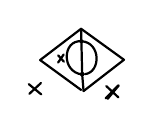
\begin{tikzpicture}[x=1em,y=1em,line cap=round,line join=round]
\draw[thick] (1.48,.04)--(0,1.12)--(1.48,2.25)--(3.03,1.13)--(1.57,0);
\draw[thick] (1.62,.61) .. controls (2.20,.68) and (2.20,1.76) .. (1.49,1.80) .. controls (.80,1.85) and (.76,.68) .. (1.52,.60);
\draw[thick] (1.48,2.25)--(1.52,.59)--(1.57,0);
\fill (1.49,1.80) circle (.074) (1.52,.61) circle (.085);
% Small internal x, then two larger external X-shaped marks.
\draw[thick] (.65,1.03)--(.85,1.32) (.65,1.29)--(.86,1.06);
\draw[thick] (-.39,-.10)--(.03,.29) (-.41,.25)--(.04,-.12);
\draw[thick] (2.37,-.26)--(2.82,.20) (2.39,.18)--(2.83,-.23);
\draw[thick] (2.44,-.28)--(2.84,.20);
\end{tikzpicture}}
\margin{Mais on aura $\unsure{X'|x'}_{L}\parallel Y'_{L}\Longrightarrow \unsure{X'|x'}\mathrel{\tikz[x=.55em,y=.60em,line cap=round]{\draw (0,-.12)--(0,1) (.48,-.12)--(.48,1) (-.06,.30)--(.54,.47) (-.05,.51)--(.53,.65);}}Y'$,\\ C'est un \unsure{contre-exple|contre-exemple|contre exemple} à l' : At $\parallel$, et a fortiori à \unsure{\deleted{ex}|ex} At 11 (cf GF $\underline{\overline{\mathrm{VI}}}$, p. 67,68)}%

% The thin vertical rule belongs beside the live axiom, not inside the title
% Critere. Ancien is an oblique interlinear word above/right of Soient;
% its verbal attachment remains uncertain although its letters are resolved.
\margin{\tikz[x=.5em,y=.5em]{\draw (0,0)--(0,4.25);}}%
\uline{At DD} 1 \tikz[baseline=(so.base)]{\node[inner sep=0pt] (so) {Soient};\node[anchor=south west,rotate=43,inner sep=0pt] at (so.north east) {\inserted{ancien}};} $X,Y\ \mathrel{\tikz[baseline=-.3ex,x=.48em,y=.65em,line cap=round]{\draw (.4,.9)..controls(-.05,.8)and(-.08,.04)..(.35,.04)..controls(.66,.04)and(.6,.6)..(.3,.63);\draw (.43,.33)--(.66,.35) (.33,.03)--(.36,-.1);}}\ X',Y'\in M$, $X\mathrel{\tikz[baseline=-.4ex,x=.65em,y=.65em]{\draw (0,1.1)--(1,.5)--(0,-.1) (1,1.1)--(0,.5)--(1,-.1);}}Y,\ X'\ll X,Y'\ll Y$. Posons $K=X\cap Y=\underset{Z\in\widetilde X\cap\widetilde Y}{\mathrm{Sup}}\,Z$. Alors $X'_{L}\mathrel{\tikz[baseline=-.4ex,x=.65em,y=.65em]{\draw (0,1.1)--(1,.5)--(0,-.1) (1,1.1)--(0,.5)--(1,-.1);}}Y'_{L}$ implique $X'\mathrel{\tikz[baseline=-.4ex,x=.65em,y=.65em]{\draw (0,1.1)--(1,.5)--(0,-.1) (1,1.1)--(0,.5)--(1,-.1);}}Y'$ \quad (NB \unsure{l'inverse|l'énoncé}\unsure{\, :|\, .|\,} \deleted{\unsure{est}} est tjrs vrai)
\normalmarginpar

\uline{Corollaire} 1 \quad \unsure{la|le} ``propriété'' ci dessus

\[
F\parallel G,\ F'\ll F,\ C'\ll G\ \Longrightarrow\ F'\parallel G'
\tag*{\makebox[0pt][r]{\makebox[\displaywidth][l]{\uline{Corollaire} 2}}}
\]

Plus gén. \quad Si $F\mathrel{\tikz[baseline=-.4ex,x=.65em,y=.65em]{\draw (0,1.1)--(1,.5)--(0,-.1) (1,1.1)--(0,.5)--(1,-.1);}}G,\ F'\ll F,\ C'\ll G$, alors
\[
 F'\parallel G'\ \Longleftrightarrow\ F'_{L}\parallel G'_{L}
\]
